\chapter{树与二叉树}
\section{树}
在\ref{sec:数据结构}节中，我们已经对“什么是树”有了一个感性的认知。与现实中的大树类似，数据结构中的树也是一种由根开始分叉生长的结构。
比如游戏中一个队长三个队员的四人小队可以看成一棵树：
\begin{bulk}
\begin{center}
\begin{tikzpicture}
[
    level distance=1.2cm,
    sibling distance=2cm
]
\node[treenode]{邪念}
    child {
        node[treenode]{银心}
    }
    child {
        node[treenode]{甘尔}
    }
    child {
        node[treenode]{张三}
    };
\end{tikzpicture}
\end{center}
\end{bulk}

你的个人计算机中目录结构的组织是一棵树：
\begin{bulk}
\begin{center}
\begin{tikzpicture}
[
    level distance=1.2cm,
    level 1/.style={
        sibling distance=6cm
    },
    level 2/.style={
        sibling distance=1.8cm
    },
    level 3/.style={
        sibling distance=1.5cm
    },
]
\node[treenode]{此电脑}
    child {
        node[treenode]{本地磁盘(C:)}
        child{
            node[treenode]{Program Files}
        }
        child{
            node[treenode]{Windows}
        }
        child{
            node[treenode]{用户}
        }
        child {
            node[treenode]{...}
        }
    }
    child {
        node[treenode]{新加卷(D:)}
        child{
            node[treenode]{电影}
            child {
                node[treenode]{泰坦尼克号}
            }
            child {
                node[treenode]{...}
            }
        }
        child{
            node[treenode]{照片}
        }
        child {
            node[treenode]{...}
        }
    };
\end{tikzpicture}
\end{center}
\end{bulk}

下面给出树的定义。
\begin{definitionbox}

    \term{树}是$n$（n>=0）个数据元素组成的有限集合，当n=0时，称为\term{空树}。任何一棵非空树都满足以下条件：
    
    \begin{enumerate}
        \item 有且仅有一个数据元素无前驱，称为\term{根节点}；
        \item 除根节点外，其余每个数据元素都有且仅有一个前驱节点，称为\term{父节点}；
        \item 每个数据元素可以有零个或多个后继节点，称为\term{子节点}。
    \end{enumerate}

\end{definitionbox}

由以上定义可知，对于一棵非空树中的任意一个节点，以该节点为根节点，连同该节点的所有后代节点在内所构成的仍是一棵树，称为原树的一棵\term{子树}。
通常认为一棵树本身是自己的子树。很少存在一些场景会关心树中节点的各个子树从左至右是否有次序（即互换后还能不能认为是同一棵树），但通常将节点有次序的树称为
\term{有序树}，节点没有次序的树称为\term{无序树}。

“树”这个逻辑结构该如何实现？如果采用链表类似的思想，每个节点除保存数据外，再保存所有指向其孩子节点的指针，像这样：
\begin{cppcode}
    struct TreeNode {
        ElemType data;
        TreeNode* child1;
        TreeNode* child2;
        TreeNode* child3;
        ...
    }
\end{cppcode}
显然，我们无法预知每个节点有多少孩子节点，因此无法为TreeNode结构定义固定数量的孩子节点指针。
熟悉C++的同学可能会想到，可以使用一个不定长数组，将节点的所有孩子指针保存到该数组中：
\begin{cppcode}
    struct TreeNode {
        ElemType data;
        std::vector<TreeNode*> childs;  // childs是一个不定长数组，childs[0], ..., childs[n]分别表示该节点的各个孩子节点指针
    }
\end{cppcode}
如图\ref{fig:用不定长数组表示树的孩子}所示。
\begin{figure}[htbp]
    \centering
    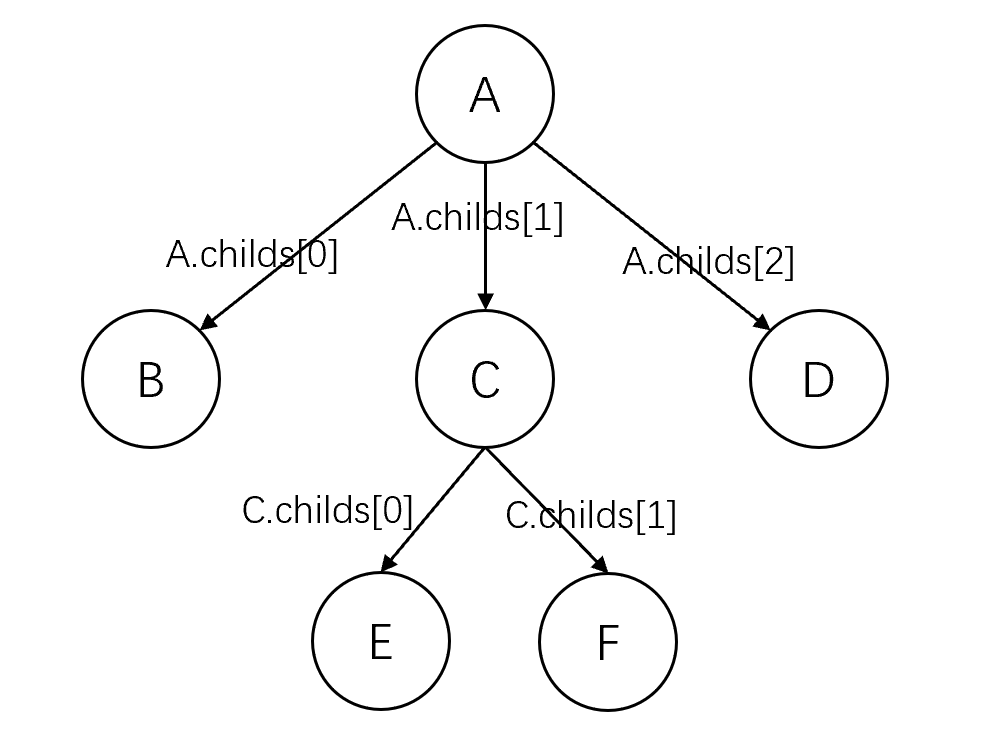
\includegraphics[width=0.47\textwidth]{assets/pics_and_ppts/ch4/树的不定长数组表示.png}
    \caption{用不定长数组表示树的孩子}
    \label{fig:用不定长数组表示树的孩子}
\end{figure}
这是完全可行，也非常自然的一种树的表示方式。但本书不要求大家熟悉C++，因此我们给出树的另一种表示方法，也是更高效的
\term{孩子-兄弟表示法（First Child - Next Sibling Representation）}。该方法存储每个节点的第一个孩子的指针，以及下一个兄弟的指针：
\begin{cppcode}
    struct TreeNode {
        ElemType data;
        TreeNode* first_child;
        TreeNode* next_sibling;
    };
\end{cppcode}
如图\ref{fig:树的孩子-兄弟表示法}所示。
\begin{figure}
    \centering
    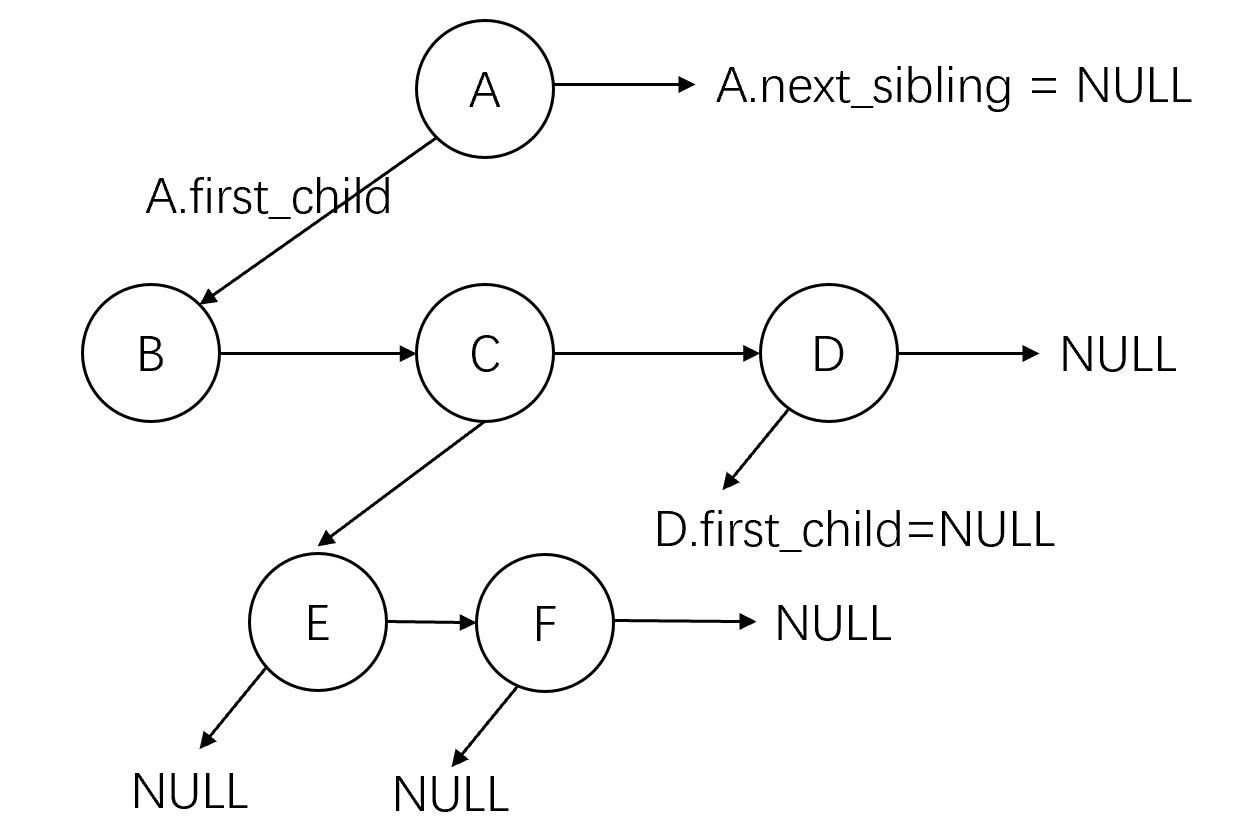
\includegraphics[width=0.6\textwidth]{assets/pics_and_ppts/ch4/树的孩子-兄弟表示法.png}
    \caption{树的孩子-兄弟表示法}
    \label{fig:树的孩子-兄弟表示法}
\end{figure}


显然该表示法下，只要拿到根节点指针，就能找到树中任何一个节点。因此，可以用根节点指针表示一棵树。如：
\begin{bulk}
    TreeNode* root; 
\end{bulk}
root这个对象既可以理解为树的根节点的指针，又可以理解为以root节点为根的一棵树。\\
\begin{notebox}{提示}
    图\ref{fig:用不定长数组表示树的孩子}与图\ref{fig:树的孩子-兄弟表示法}逻辑上是同一棵树，只不过物理指针的含义不同。
\end{notebox}


有了以上的内容介绍，我们来做一点有意思的事情（当然你大可以放心地跳过）：用孩子-兄弟表示法尝试实现操作系统的目录树。

\subsection{*目录树的简单实现}
我们已经知道，操作系统对目录的管理其实就是一棵树。用户随时可能在任何目录新建目录、删除某个目录，我们暂且不考虑文件。并假设目录节点的“数据”只有一个字符串
类型的成员，表示目录的名字，如“电影”等。以下代码实现了简单的新建目录、删除目录的操作，具体过程请结合注释。

\begin{cppcode}
    // 在目录Dad中，新建一个名为name的目录
    void DirInsert(TreeNode* Dad, char* name) {
        // 函数实现：创建一个新节点，将其加入Dad的孩子链表末尾
        TreeNode* new_node = (TreeNode*)malloc(sizeof(TreeNode));
        strcpy(new_node->name, name);
        new_node->first_child = NULL;
        new_node->next_sibling = NULL;

        // Dad原本是空目录，则需要更改first_child指针。
        if(Dad->first_child == NULL) {
            Dad->first_child = new_node;
            return;
        }

        // 原本不是空目录，修改next_sibling指针。
        TreeNode* last_child = Dad->first_child;
        while(last_child->next_sibling != NULL) {
            last_child = last_child->next_sibling;
        }
        last_child->next_sibling = new_node;
        return;
    }

    // 销毁一个节点及其所有后代
    void DestroyTree(TreeNode* root) {
        if(root == NULL) return;
        // 先递归销毁其子树
        DestroyTree(root->first_child);

        // 再释放根节点
        free(root);
    }

    // 在目录Dad中，删除目录to_del
    void DirDelete(TreeNode* Dad, TreeNode* to_del) {
        // 函数实现：先把to_del从父节点的孩子链表中摘掉，再销毁以to_del为根的整棵树
        if(Dad == NULL) {
            return;
        }
        // 要删除的就是第一个孩子节点，需要更新first_child指针
        if(to_del == Dad->first_child) {
            Dad->first_child = to_del->next_sibling;;
            // 注意这里不能简单地free(to_del)，因为该目录中可能还有若干目录，目录中可能还有目录，因此要递归销毁。
            DestroyTree(to_del);
            return;
        }

        // 找到要删除的节点的前一个兄弟节点
        TreeNode* pre = Dad->first_child;
        while(pre->next_sibling != to_del) {
            pre = pre->next_sibling;
        }

        // 修改链条，类似单链表的删除操作
        pre->next_sibling = to_del->next_sibling;
        // 注意同样要递归销毁
        DestroyTree(to_del);
        return;
    }
\end{cppcode}

\begin{notebox}{提示}
    以上例子也给了我们一个重要提示：树中每个节点的子节点很多时候不能单纯的看成一个节点，而是要看成一棵子树。因此与树相关的操作，很多都会涉及到递归，这一点非常重要。
\end{notebox}

\subsection{树的一些基本概念}
我们回到逻辑上的数据结构：树。树中有一些大家常用的专业术语与性质，我们在这里列出。\\
\begin{figure}
    \centering
    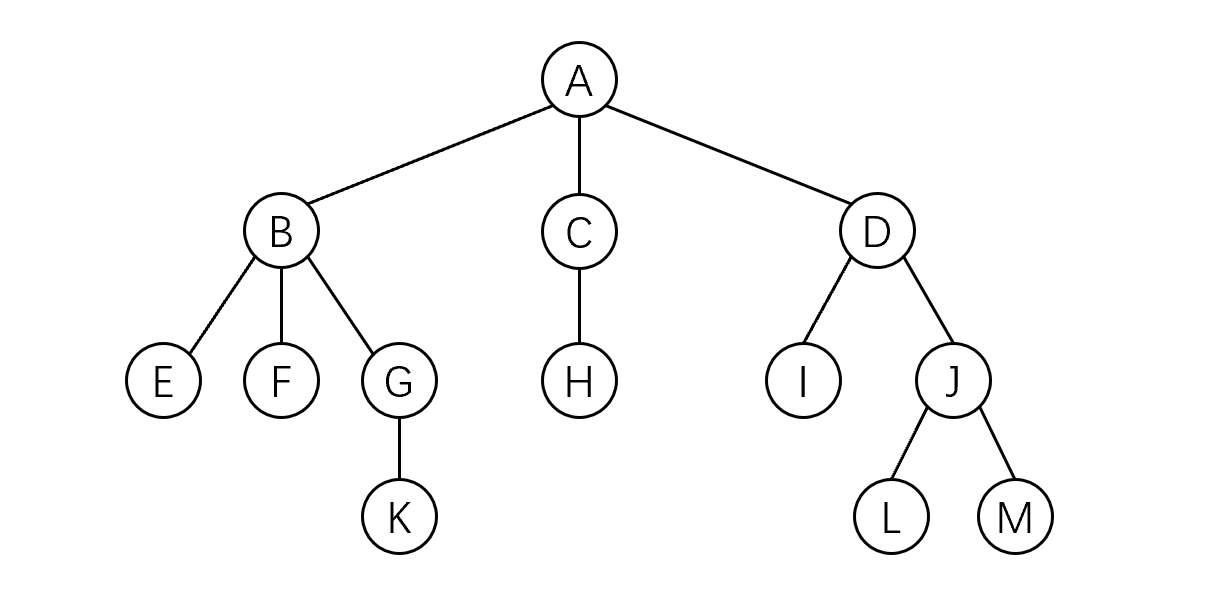
\includegraphics[width=0.6\textwidth]{assets/pics_and_ppts/ch4/一棵树.png}
    \caption{}
    \label{fig:一棵树}
\end{figure}

a）树中，一个节点拥有的子树数量称为\term{节点的度}。一棵树中所有节点的度的最大值称为这棵\term{树的度}。

b）树中度为0的节点称为\term{叶子节点}，简称\term{叶节点}。显然叶节点没有孩子节点。不是叶子节点的节点称为\term{非叶节点}。\\
图\ref{fig:一棵树}中，节点A、B的度均为3，整棵树的度为3；节点E、F、K、H、I、L、M的度为0，是叶子节点。\\
c）可以看出树是一种具有层次结构的数据结构。根节点处于最高层，通常定义根为第1层，根的孩子为第2层。若某节点处在第i层，其子树的根节点就处在第i+1层。

d）\term{节点的深度}通常定义为节点的所在层次；而\term{节点的高度}通常是指从最底层叶子节点（高度为1）开始逐层累加至该节点时的高度值。所有节点的深度
的最大值称为\term{树的深度}或\term{树的高度}。即
\begin{bulk}
    \begin{center}
        树的高度 = max\{所有节点的深度值\} = max\{所有节点的高度值\}
    \end{center}
\end{bulk}

图\ref{fig:一棵树}中，节点A的深度为1，高度为4；节点B的深度为2，高度为3；节点K的深度为4，高度为1。整棵树的深度，或称整棵树的高度，为4。

\begin{notebox}{提示}
    1.有些人喜欢将根节点的高度定义为0，本书若无特别说明，默认按照根节点高度为1来定义。\\
    2.注意区分节点与树的深度和高度：节点的高度和节点的深度通常不是一回事；而树的高度和树的深度一定是相等的。
\end{notebox}


\section{二叉树}
很少有实际问题需要直接通过二叉树来解决，但是二叉树在计算机科学中的应用是非常非常重要的。许多更加有用的数据结构都是一棵二叉树。而且对二叉树的研究可以为我们建立
类似树的层次结构的思维方式。笔者认为，对“二叉树”的研究在整个《数据结构》中都是相当重要的。
\begin{definitionbox}
    \term{二叉树}要么是一棵空树，要么是一棵：\\
    
    由根节点以及它的两棵子树构成的树，这两棵子树有左右位置之分，分别称为\term{左子树}和\term{右子树}，并且左子树和右子树依然是一棵二叉树。
\end{definitionbox}
可以看到，二叉树是\term{递归定义}的，即用二叉树自身来定义二叉树。
如图\ref{fig:几棵不同的二叉树}所示的几棵树都是二叉树，根据图中文字介绍，大家也能进一步体会二叉树的递归定义。
\begin{figure}
    \centering
    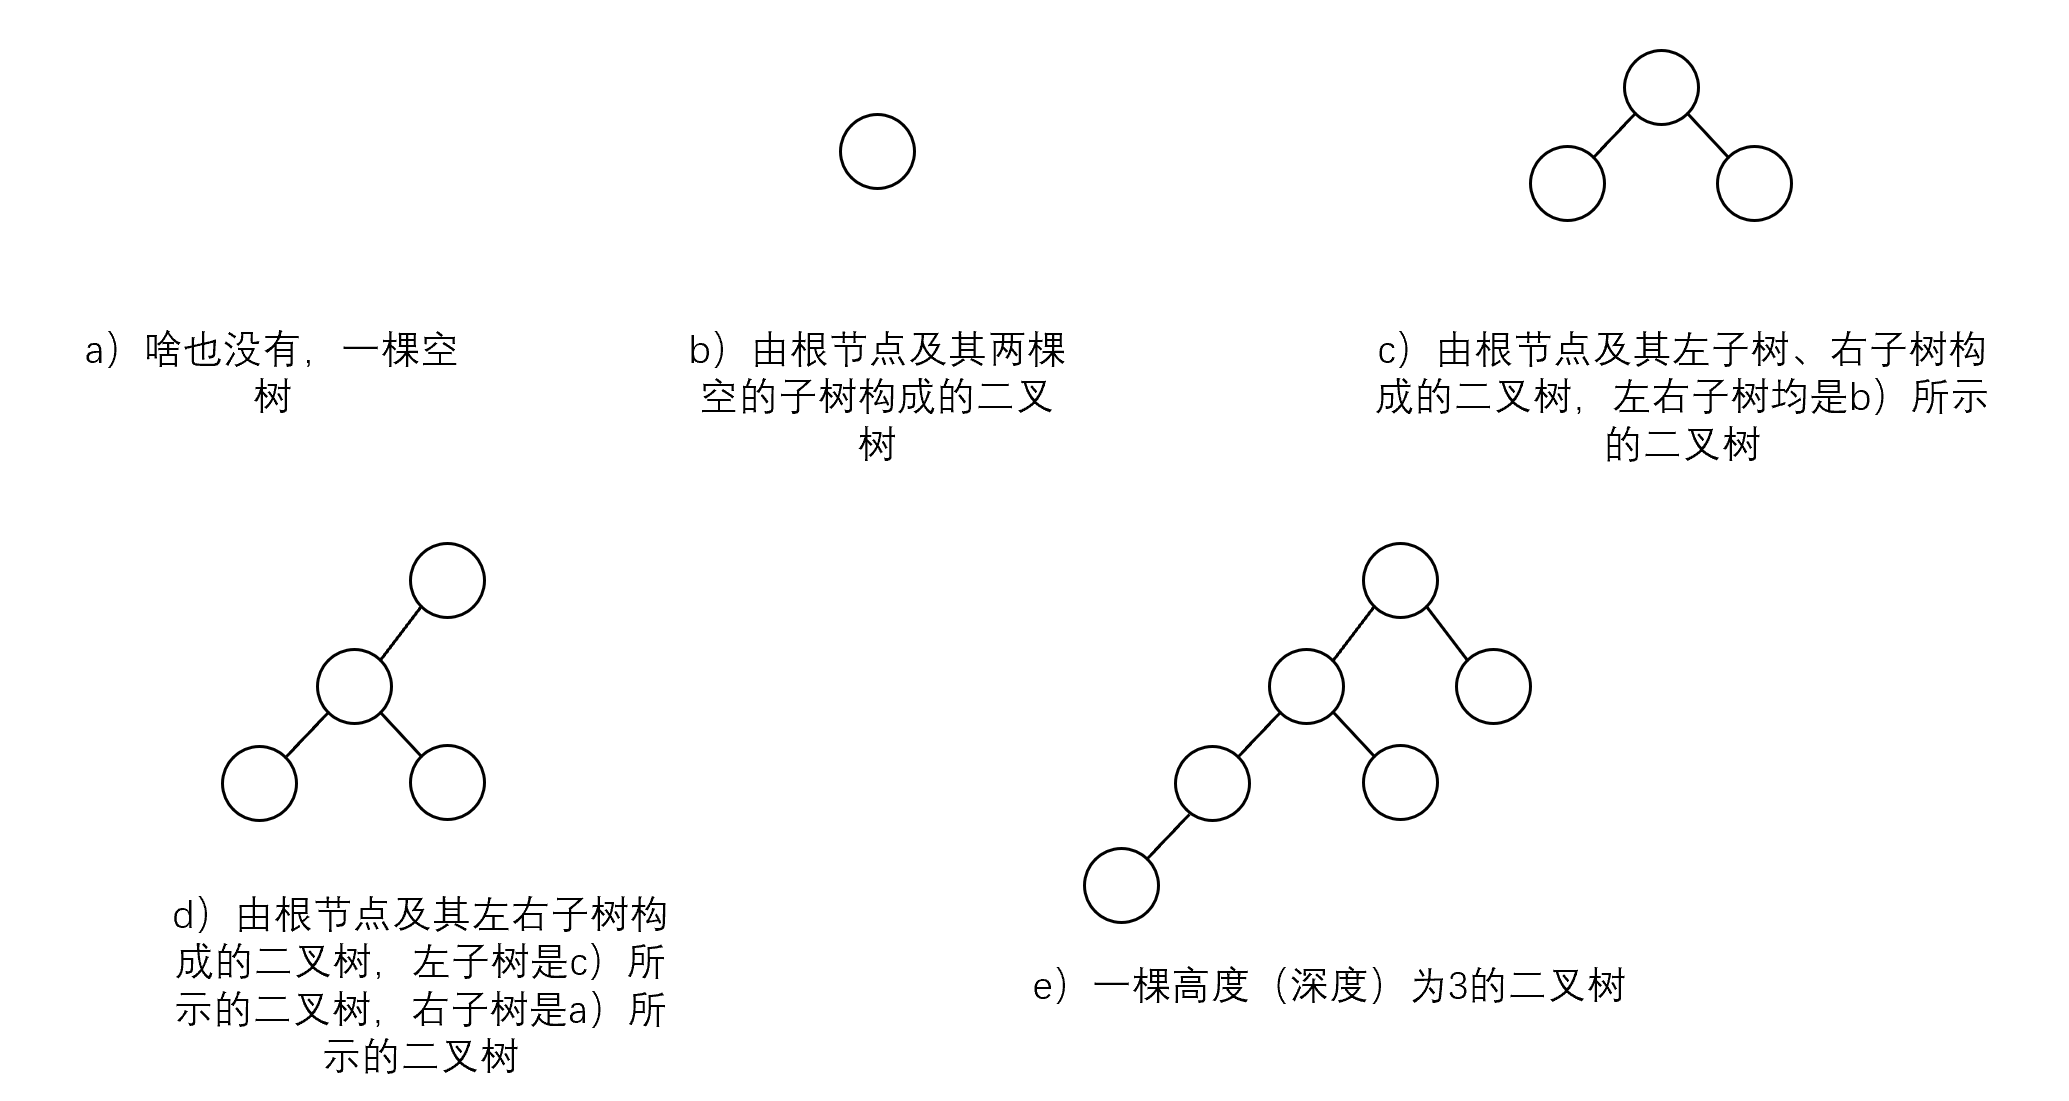
\includegraphics[width=1.0\textwidth]{assets/pics_and_ppts/ch4/几棵不同的二叉树.png}
    \caption{几棵不同的二叉树}
    \label{fig:几棵不同的二叉树}
\end{figure}

显然二叉树的度只可能是0、1或2，二叉树中每一个节点的度也只可能是0、1或2。



\begin{notebox}{提示}
    “二叉树”与“度为2的有序树”有如下区别：\\
    1. 度为2的树至少有3个节点，而二叉树未必；\\
    2. 二叉树即使只有一个孩子节点，该节点也要区分左右。而度为2的有序树，其“有序”是兄弟之间的位置有序，若某个节点是“独生子女”，则其位置是唯一确定的，不分左右。
    二叉树明确区分孩子的左右位置，这是因为在更多的场景下这是有用的，在后面的内容中我们将有所体会。
\end{notebox}

